\chapter{Interviews}

Um Bedürfnisse realer Benutzer von vorne herein zu Berücksichtigen haben wir mit Usern ein, durch ein Fragebogen begleitetes Interview durchgeführt.

\section{Fragebogen und Ergebnisse}

Folgende Informationen haben wir mittels eines Fragebogens abgefragt.

\subsection{Frage 1: Benutzt du Weekly Standups?}
\begin{figure}[H]
	\centering
	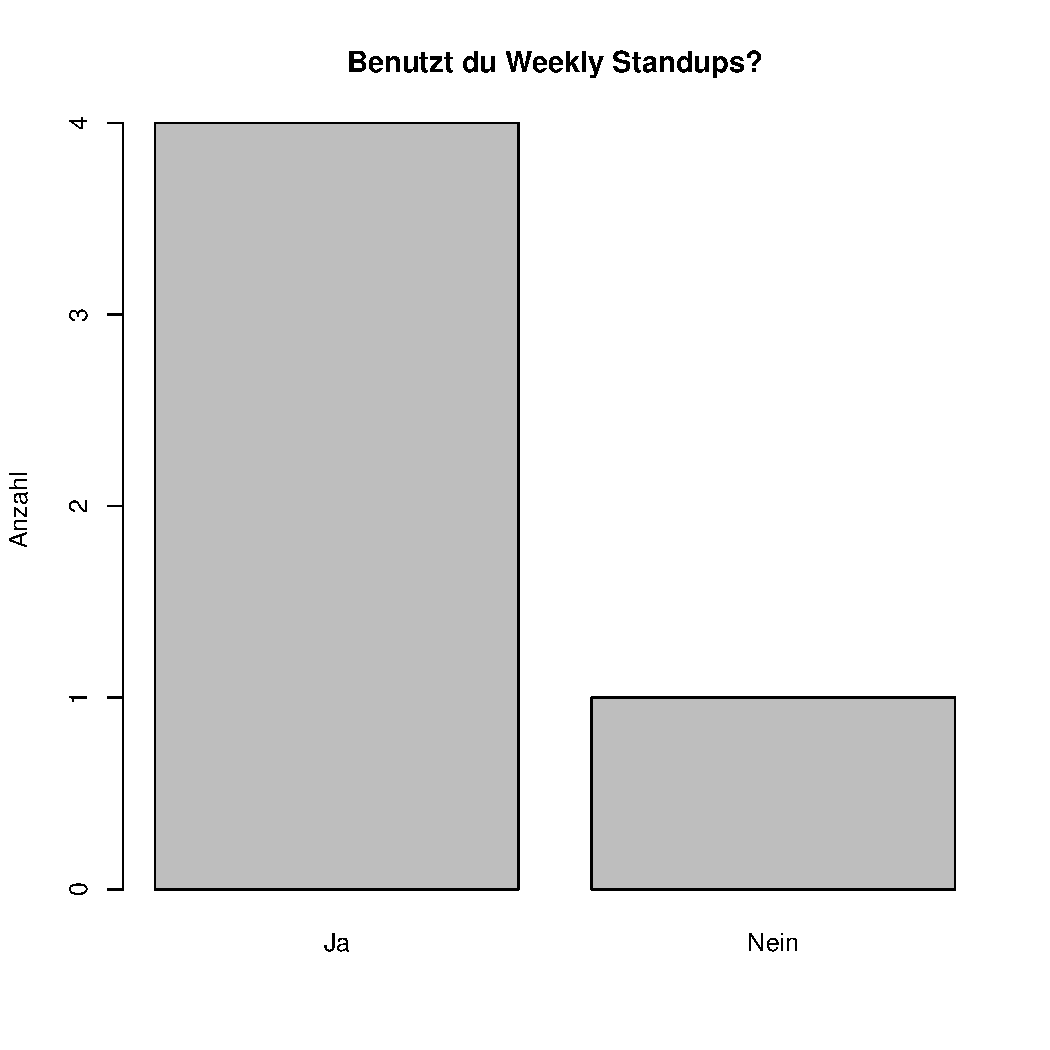
\includegraphics[width=0.60\textwidth]{q1.pdf}
    \caption{Verwendung von Weekly Standups unter den Befragten}
	\label{fig:q1}
\end{figure}

\subsection{Frage 2: Welcher Nutzergruppe gehörst du an?}
\begin{figure}[H]
	\centering
	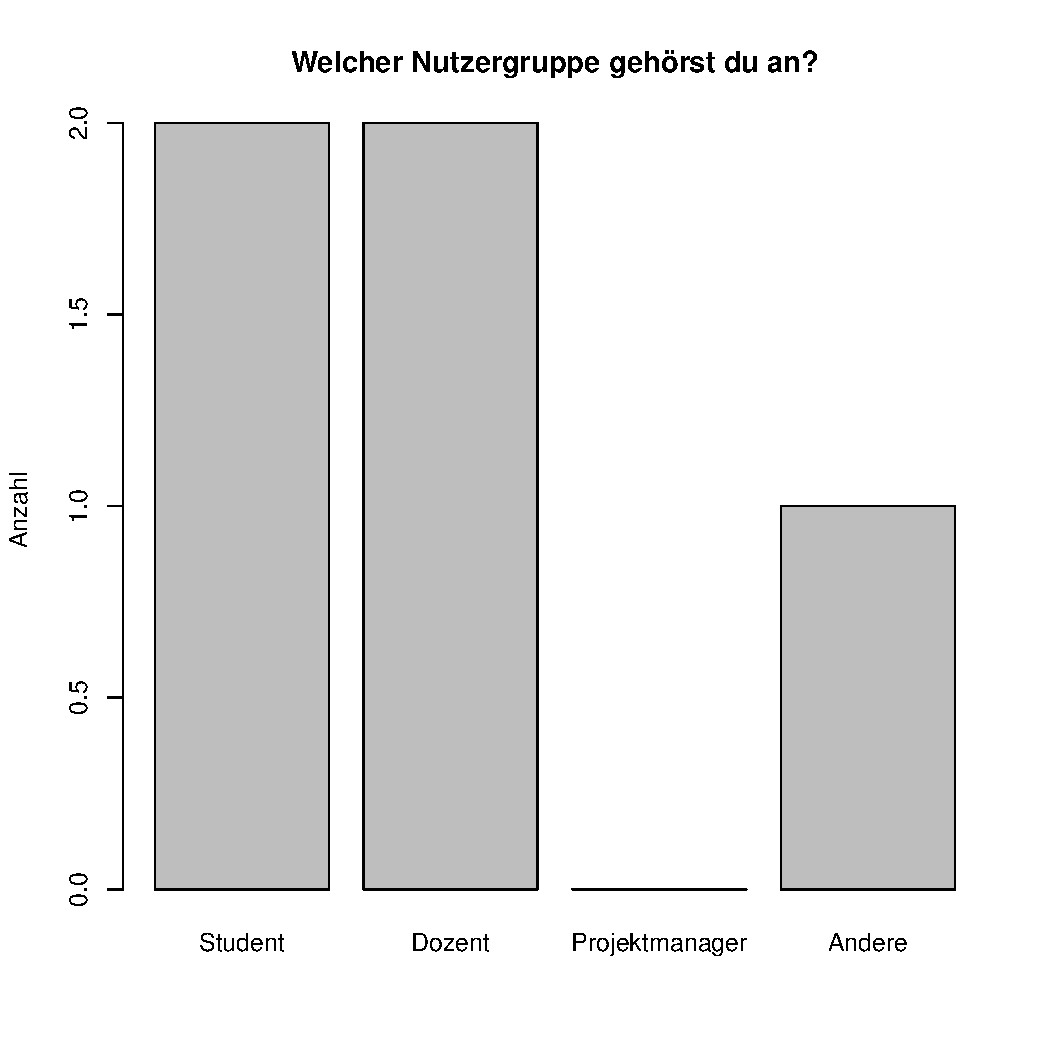
\includegraphics[width=0.60\textwidth]{q2.pdf}
    \caption{Nutzergruppe der Befragten}
	\label{fig:q2}
\end{figure}
\subsection{Frage 3: Welche Projektarten führst du aus?}
\begin{figure}[H]
	\centering
	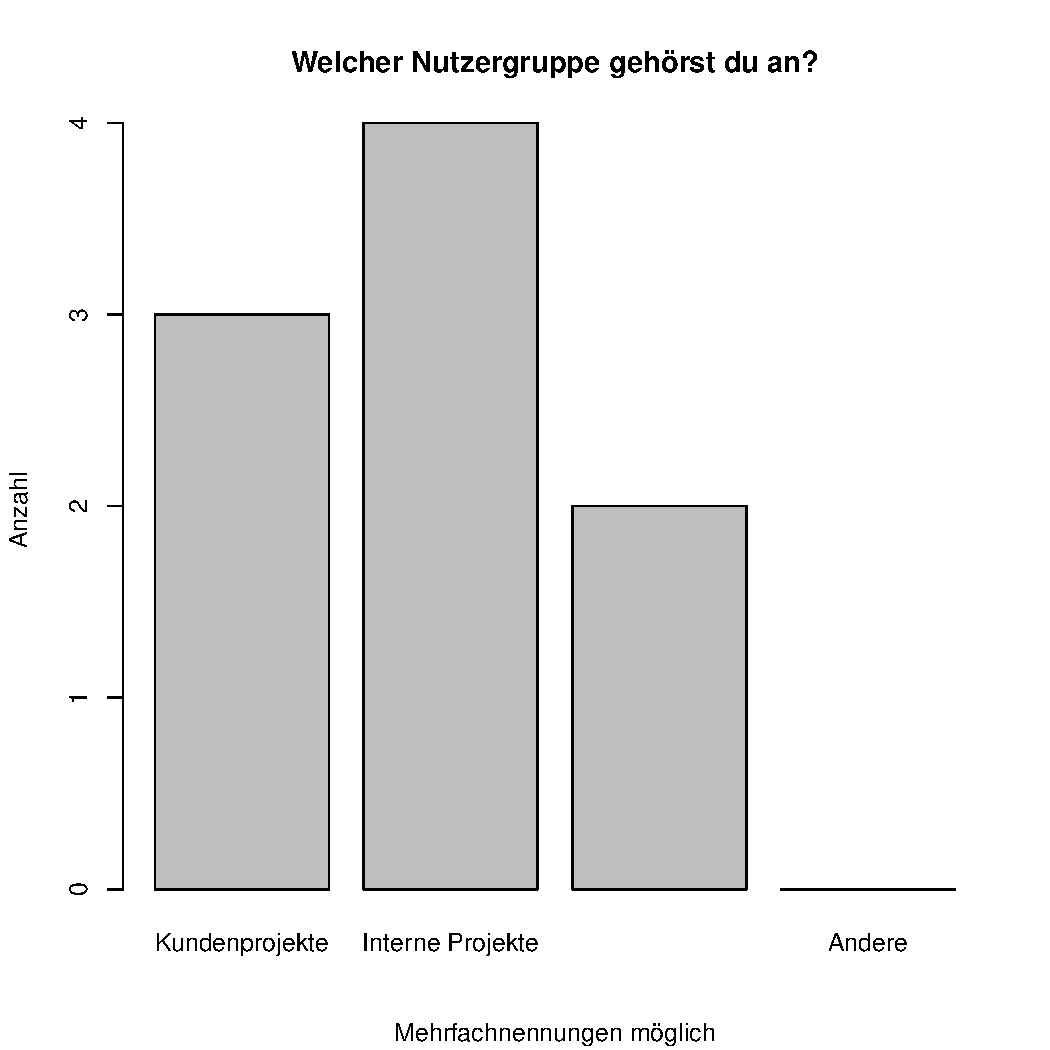
\includegraphics[width=0.60\textwidth]{q3.pdf}
    \caption{Projektarten der Befragten}
	\label{fig:q3}
\end{figure}
\subsection{Frage 4: Wie alt bist du?} 
\begin{figure}[H]
	\centering
	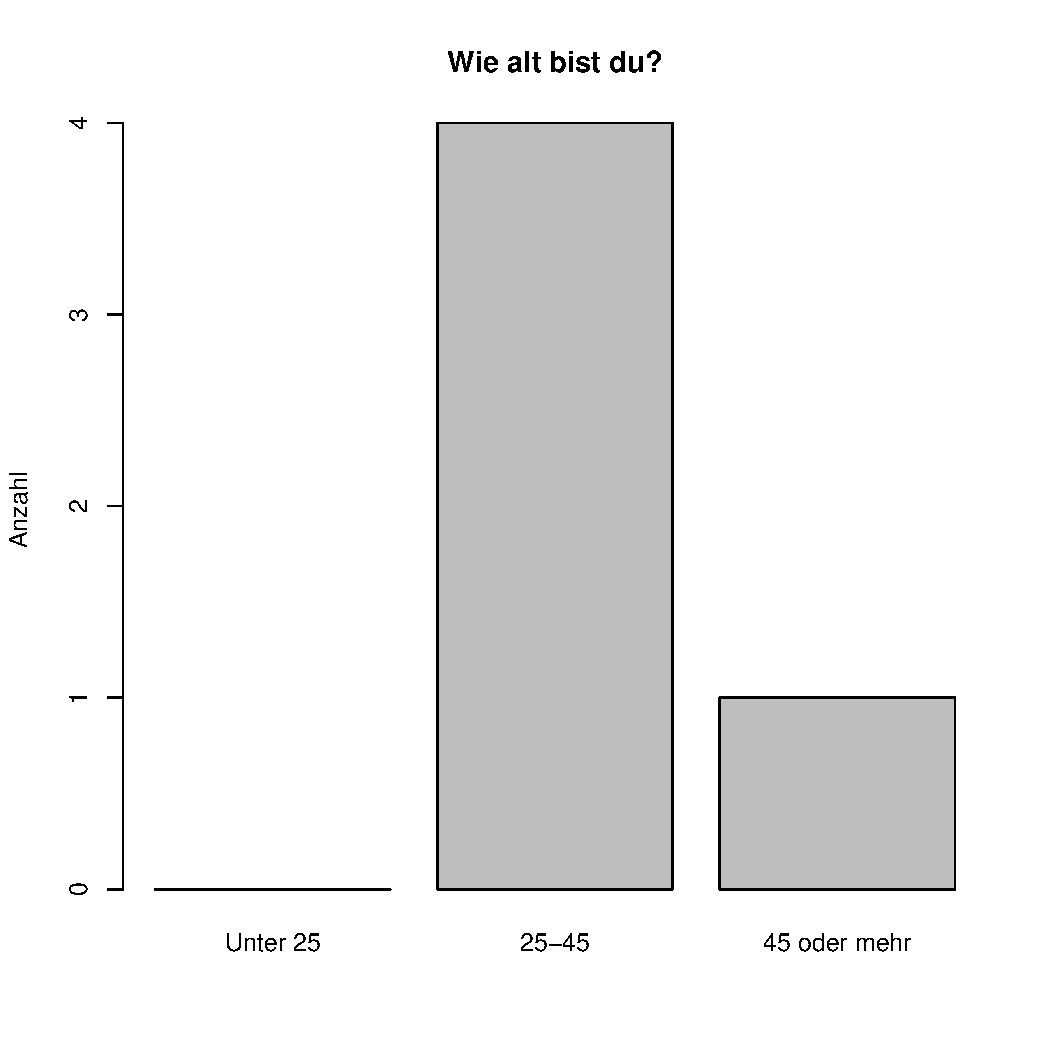
\includegraphics[width=0.60\textwidth]{q4.pdf}
    \caption{Alter der Befragten}
	\label{fig:q4}
\end{figure}     
\subsection{Frage 5: Wie viel Zeit verbringst du Wöchentlich in Standup Meetings?}
\begin{figure}[H]
	\centering
	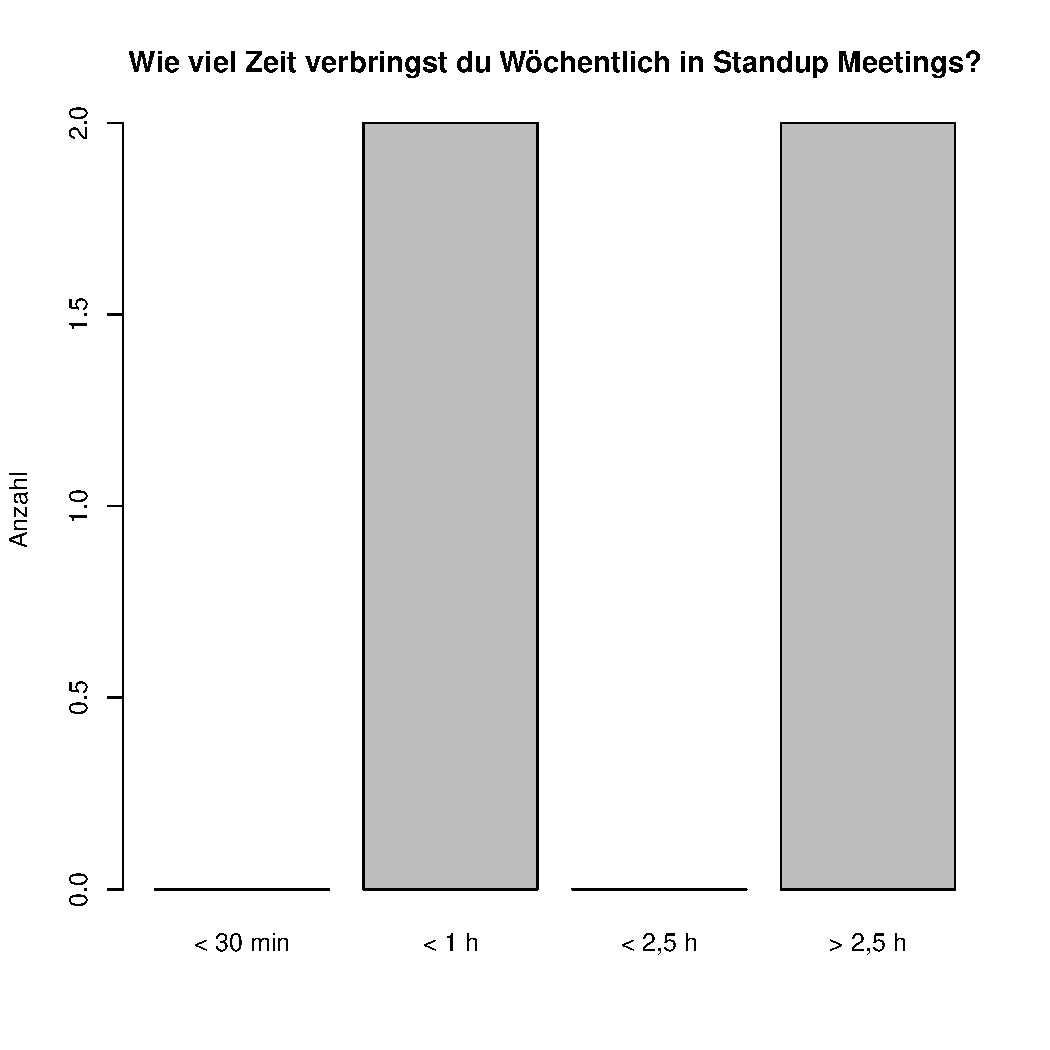
\includegraphics[width=0.60\textwidth]{q5.pdf}
    \caption{Zeit welche die Befragten in Statusmeetings verbringen}
	\label{fig:q5}
\end{figure}  
\subsection{Frage 6: Wie hilfreich findest du Weekly Standups?}
\begin{figure}[H]
	\centering
	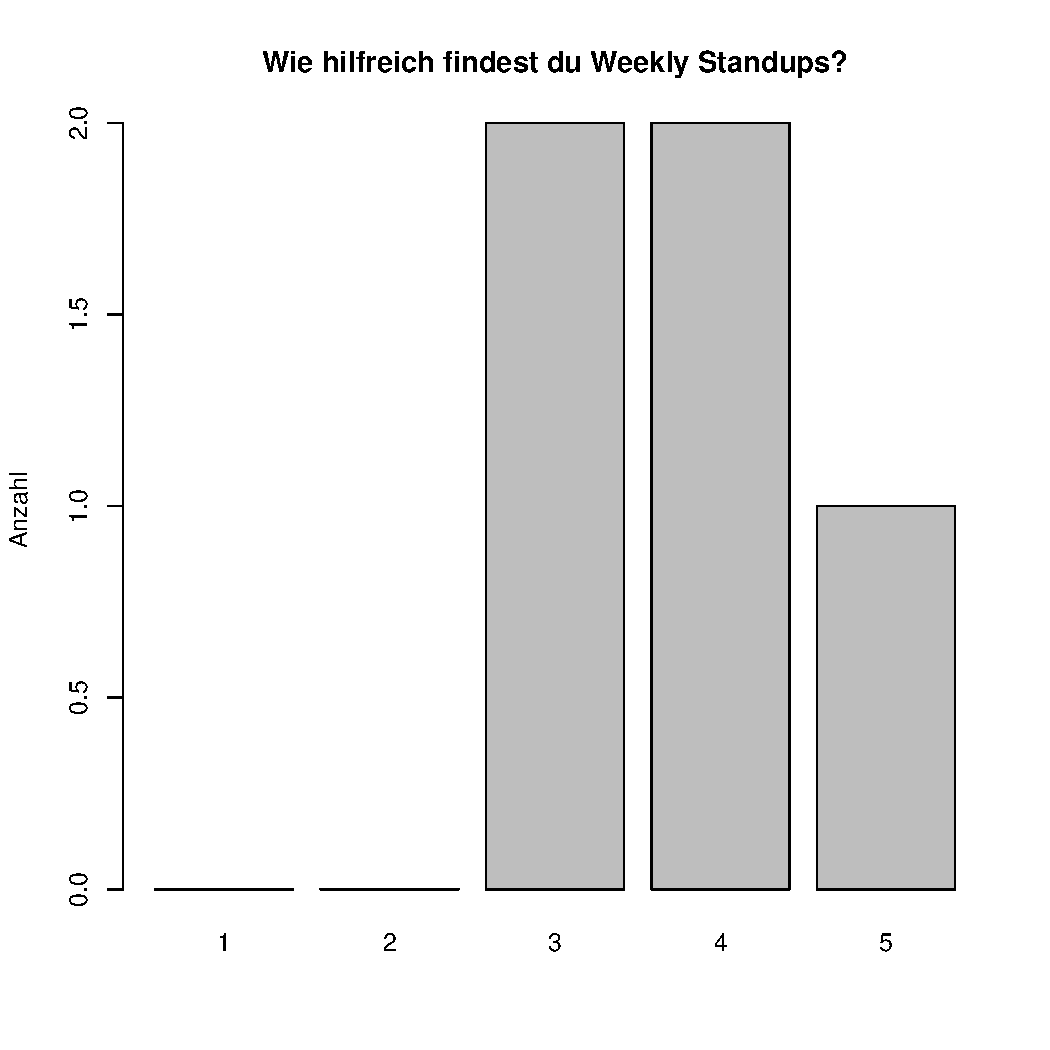
\includegraphics[width=0.60\textwidth]{q6.pdf}
    \caption{Gefühlter Nutzen eines Weekly Standups}
	\label{fig:q6}
\end{figure}  
\subsection{Frage 7: Wie arbeitest du zur Zeit?}
\begin{figure}[H]
	\centering
	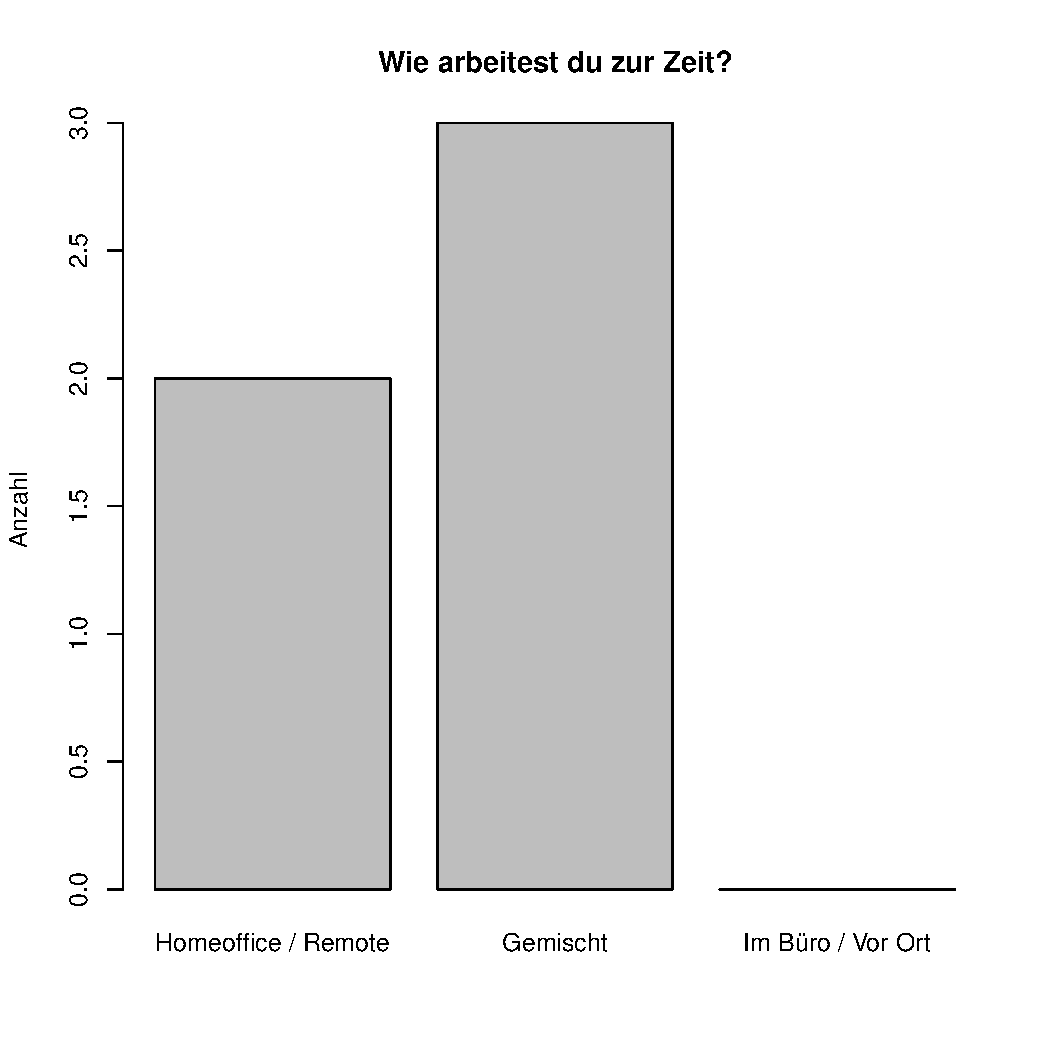
\includegraphics[width=0.60\textwidth]{q7.pdf}
    \caption{Arbeitsumfeld der Befragten}
	\label{fig:q7}
\end{figure}  
\subsection{Frage 8: Wie bewertest du folgende Features?}
\subsubsection{Frage 8.1: Erinnerung}
\begin{figure}[H]
	\centering
	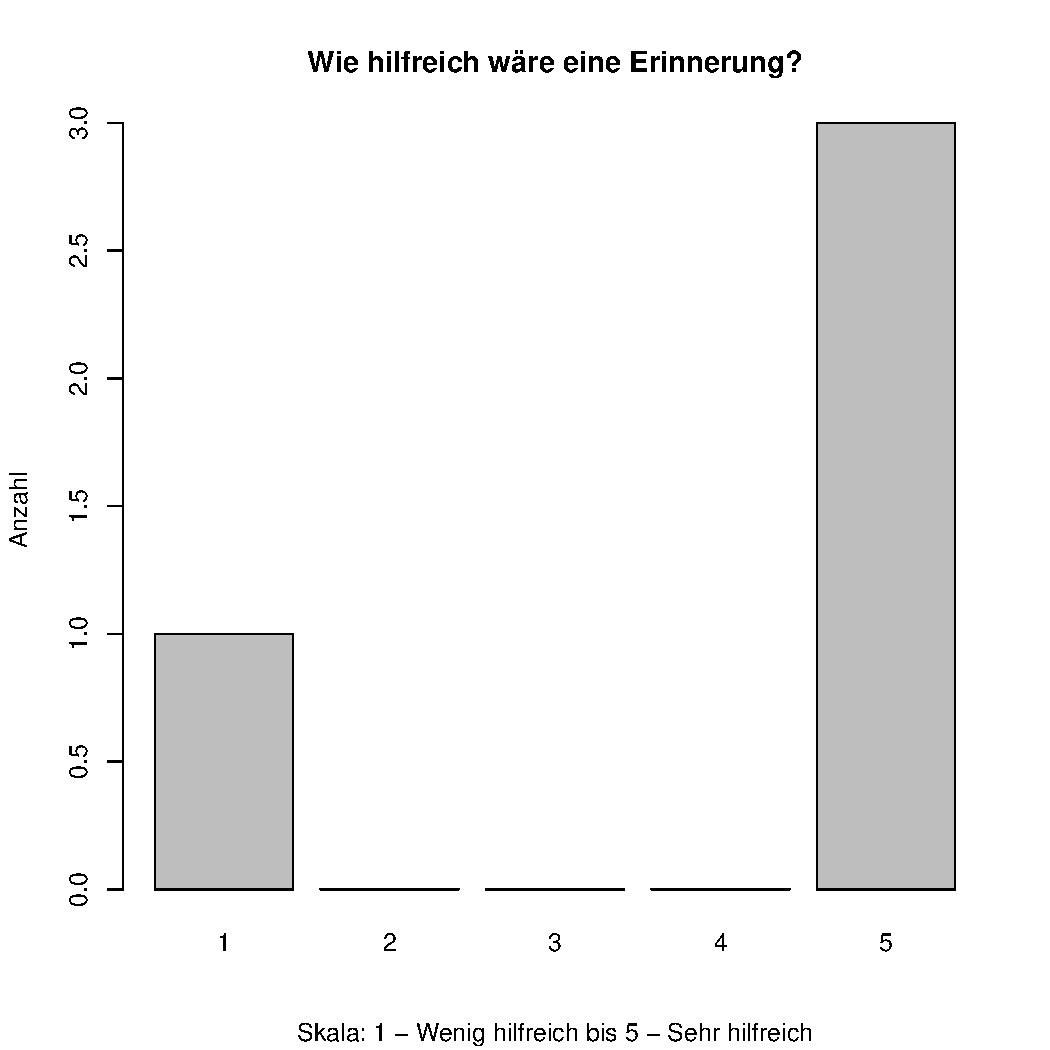
\includegraphics[width=0.60\textwidth]{q8-1.pdf}
    \caption{Nützlichkeit einer Erinnerung}
	\label{fig:q81}
\end{figure} 
\subsubsection{Frage 8.2: Timeline}
\begin{figure}[H]
	\centering
	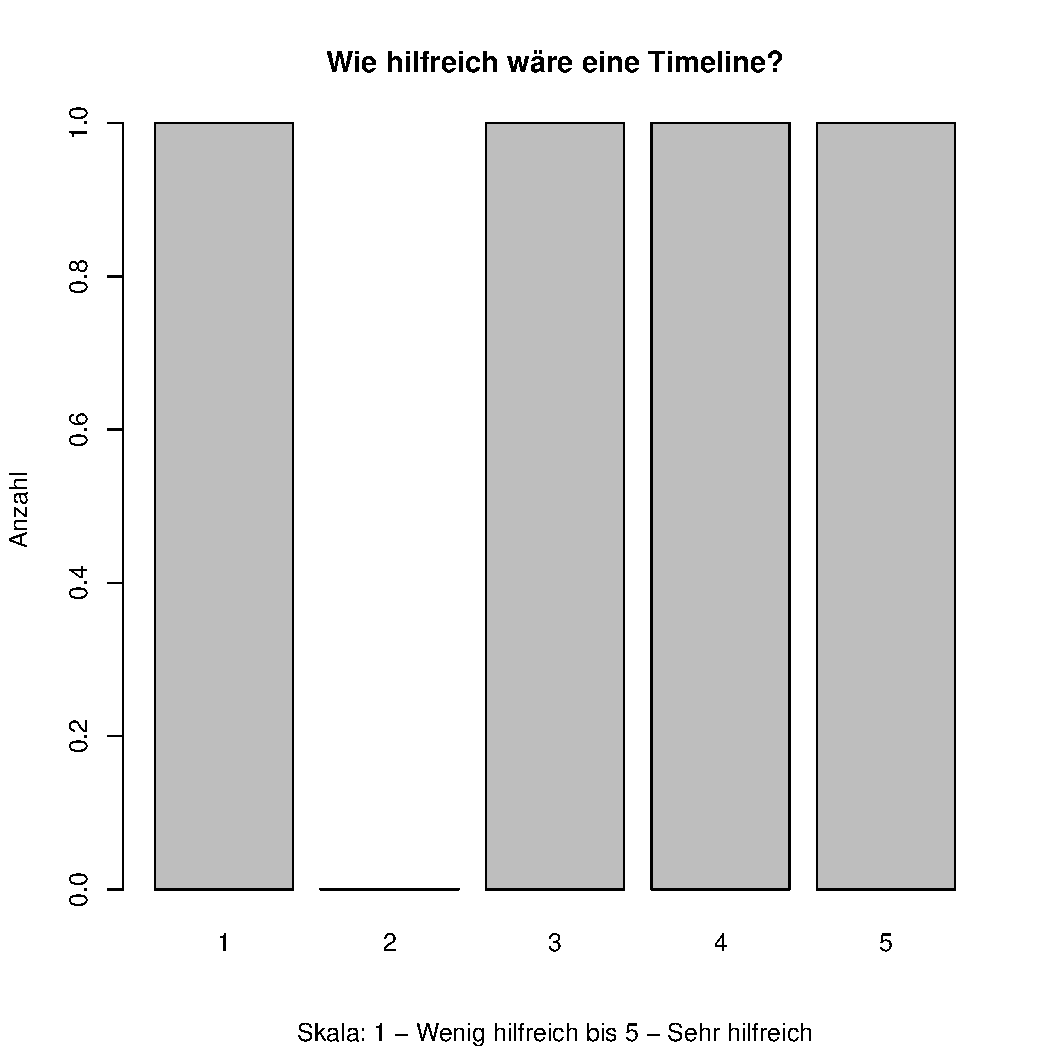
\includegraphics[width=0.60\textwidth]{q8-2.pdf}
    \caption{Nützlichkeit einer Timeline}
	\label{fig:q82}
\end{figure} 
\subsubsection{Frage 8.3: Suche}
\begin{figure}[H]
	\centering
	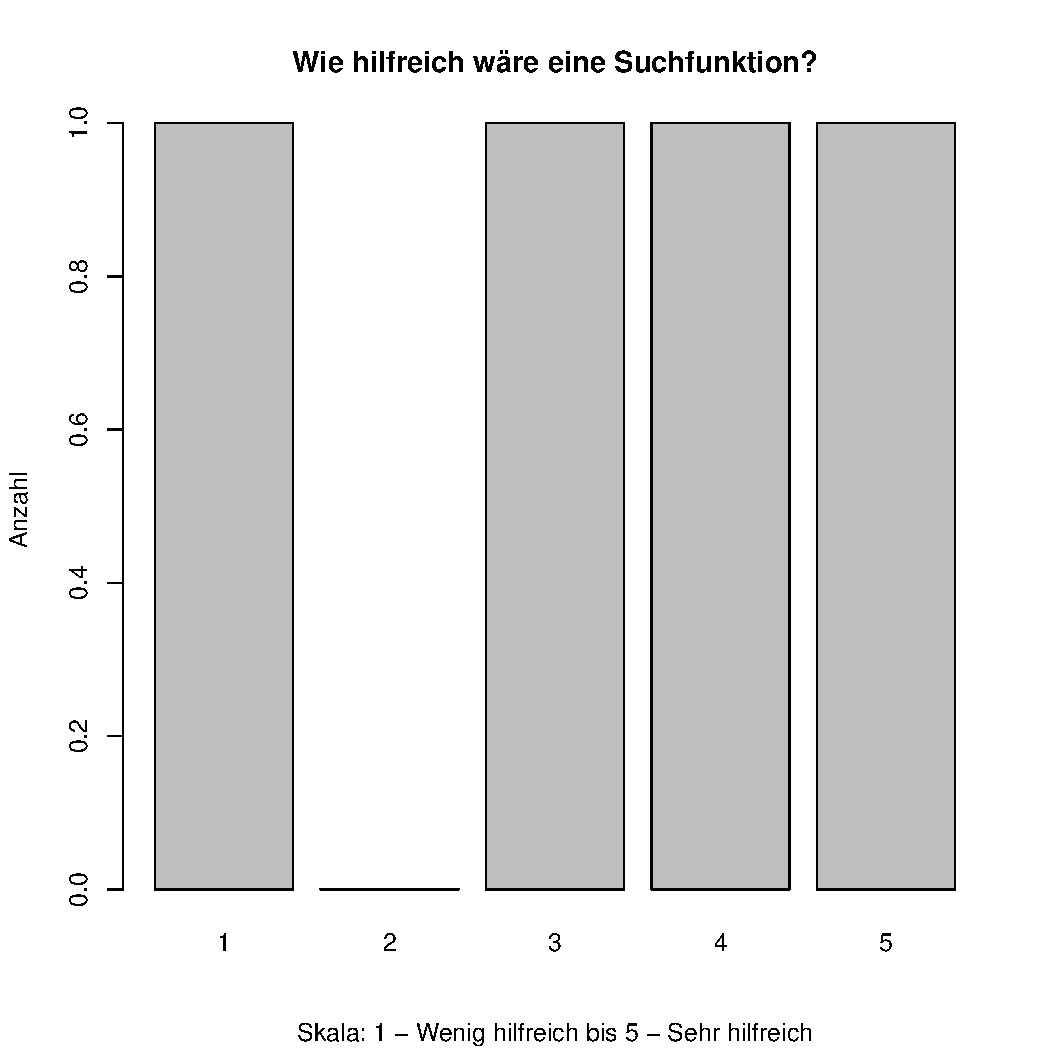
\includegraphics[width=0.60\textwidth]{q8-3.pdf}
    \caption{Nützlichkeit einer Suche}
	\label{fig:q83}
\end{figure} 
\subsubsection{Frage 8.4: Markieren}
\begin{figure}[H]
	\centering
	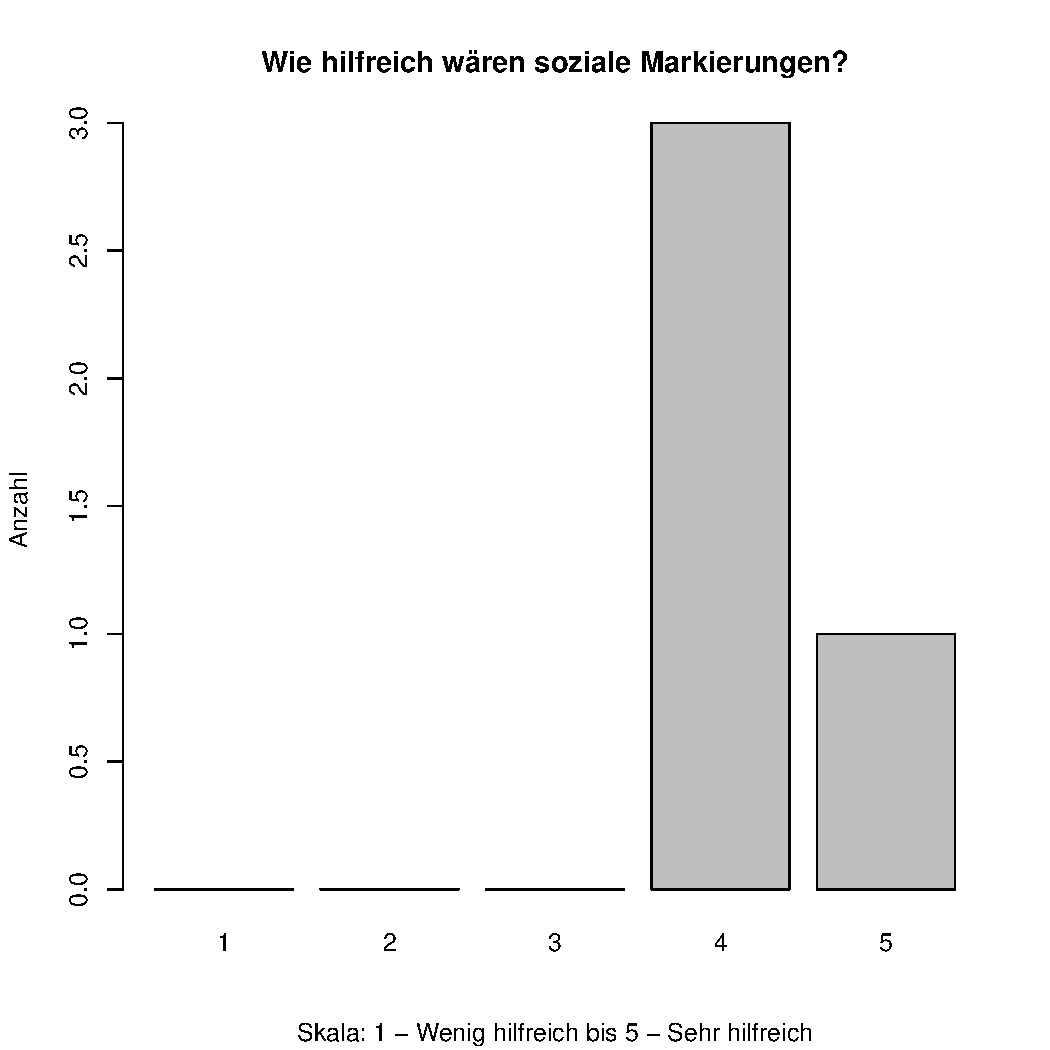
\includegraphics[width=0.60\textwidth]{q8-4.pdf}
    \caption{Nützlichkeit von Markierungen}
	\label{fig:q84}
\end{figure} 
\subsubsection{Frage 8.5: Vorgegebene Eingabefelder}
\begin{figure}[H]
	\centering
	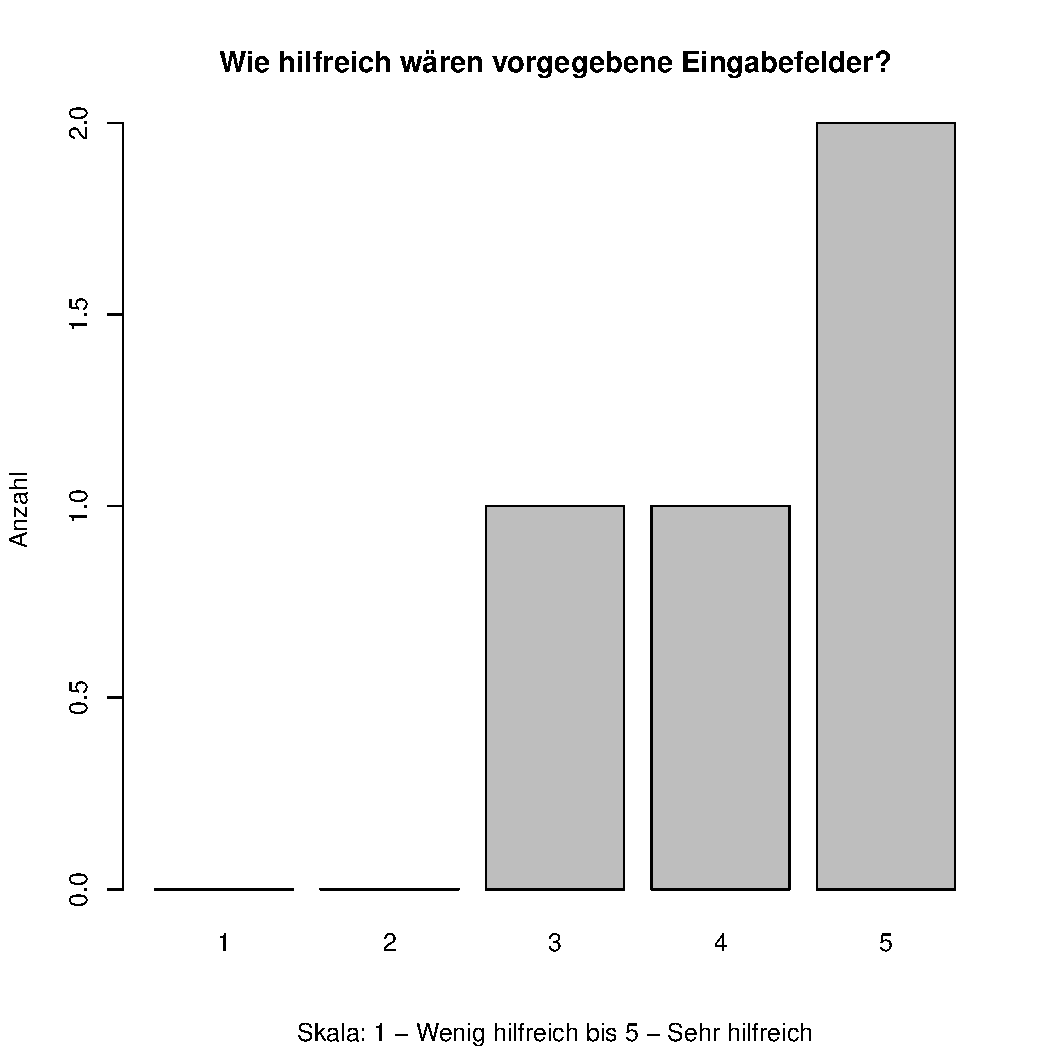
\includegraphics[width=0.60\textwidth]{q8-5.pdf}
    \caption{Nützlichkeit von Vorgaben}
	\label{fig:q85}
\end{figure} 
\subsection{Frage 9: Was ist dein bevorzugter Zeitpunkt für ein Weekly Standup?}
\begin{figure}[H]
	\centering
	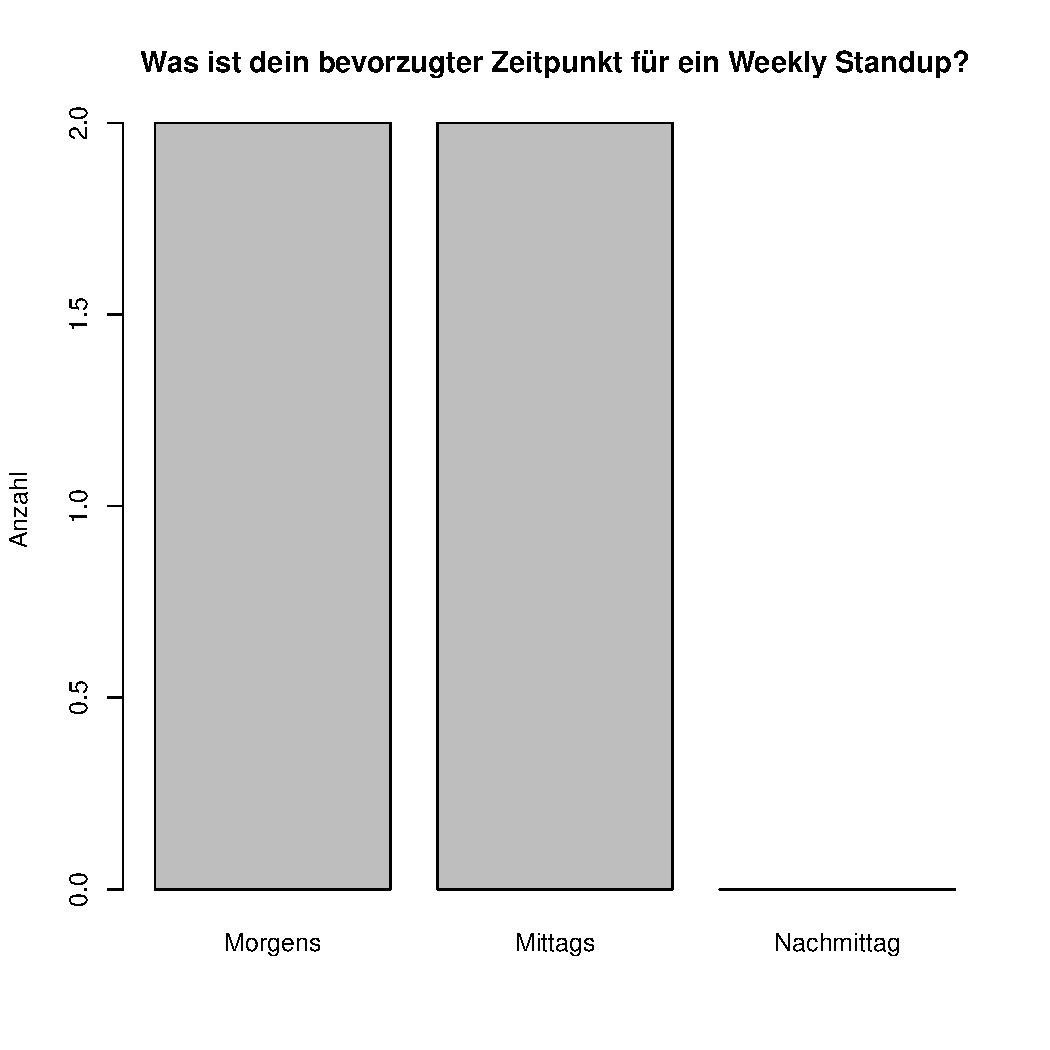
\includegraphics[width=0.60\textwidth]{q9.pdf}
    \caption{Idealer Zeitpunkt für ein Weekly Standup}
	\label{fig:q9}
\end{figure}  
\subsection{Frage 10: Welche Form eines Weekly Standups würdest du bevorzugen?}
\begin{figure}[H]
	\centering
	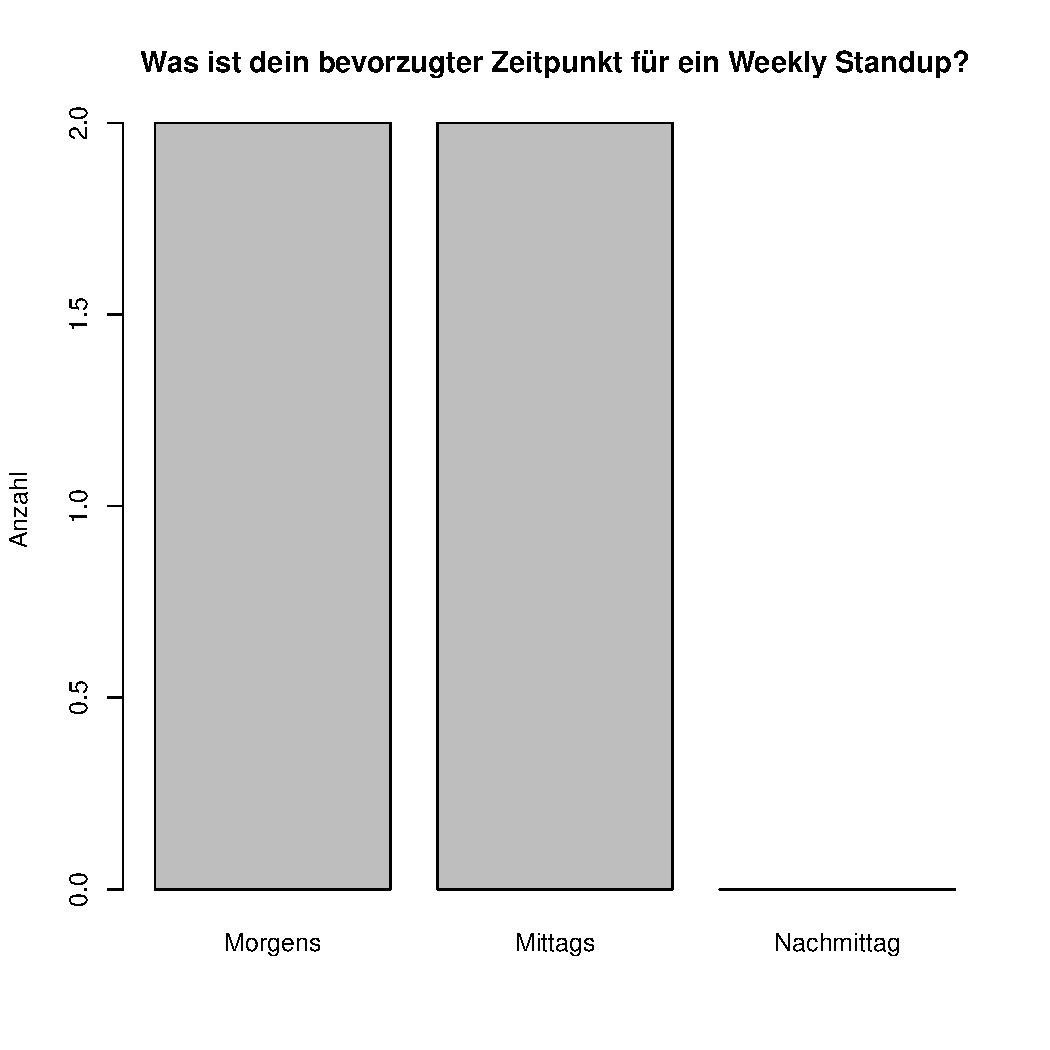
\includegraphics[width=0.60\textwidth]{q9.pdf}
    \caption{Bevorzugte form des Weekly Standups}
	\label{fig:q10}
\end{figure} 
\subsection{Frage 11: Würdest du einen Chatbot als hilfreich empfinden, welcher dir Informationen wie Deployment, Status, Logereignisse im Meeting mitteilt?}
\begin{figure}[H]
	\centering
	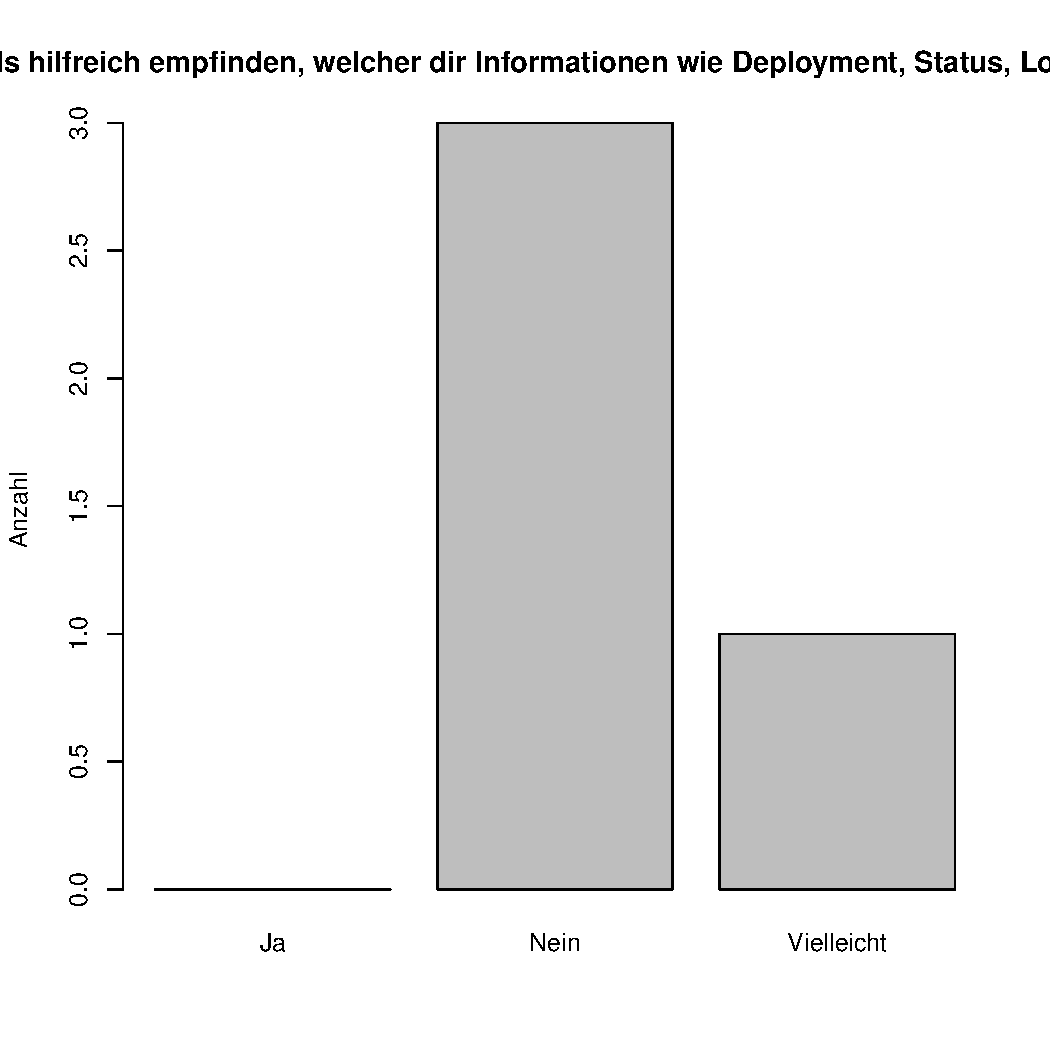
\includegraphics[width=0.60\textwidth]{q11.pdf}
    \caption{Meinung zu einem Chatbot}
	\label{fig:q11}
\end{figure} 
\subsection{Frage 12: Welche Informationen wären für dich als Projektmanager in einem Weekly Standup wichtig?}
Diese Frage wurde als Freitextaufgabe gestellt. Zwei der befragten haben sich dazu geäußert und folgende Informationen als wünschenswert zu erheben herausgestellt:
\begin{itemize}
\item Verknüpfung zu Aufgaben -> Überblick in Bezug auf den Plan
\item Muss ich als Dozent / PM intervenieren / Resourcen / Unterstützung / Hilfestellungen bereitstellen? 
\item Wer macht / wie viel mit? 
\item Gibt es Abwesenheiten?
\end{itemize}

\subsection{Frage 13: Wenn du bereits Weekly Standups gemacht hast, welche Tools hast du dafür benutzt?}
Bei dieser Frage handelte es sich wiederum um eine Freitext eingabe. die am häufigsten genannten Tools waren hierbei:
\begin{itemize}
    \item Jira (3x)
    \item Teams (3x)
    \item Miro
    \item Jitsi
\end{itemize}
Aber auch dinge wie Azure Devops oder digitale/smarte Whiteboards wurden genannt.

\subsection{Frage 14: Wie wichtig wäre dir eine Zeitbegrenzung des Meetings?}
\begin{figure}[H]
	\centering
	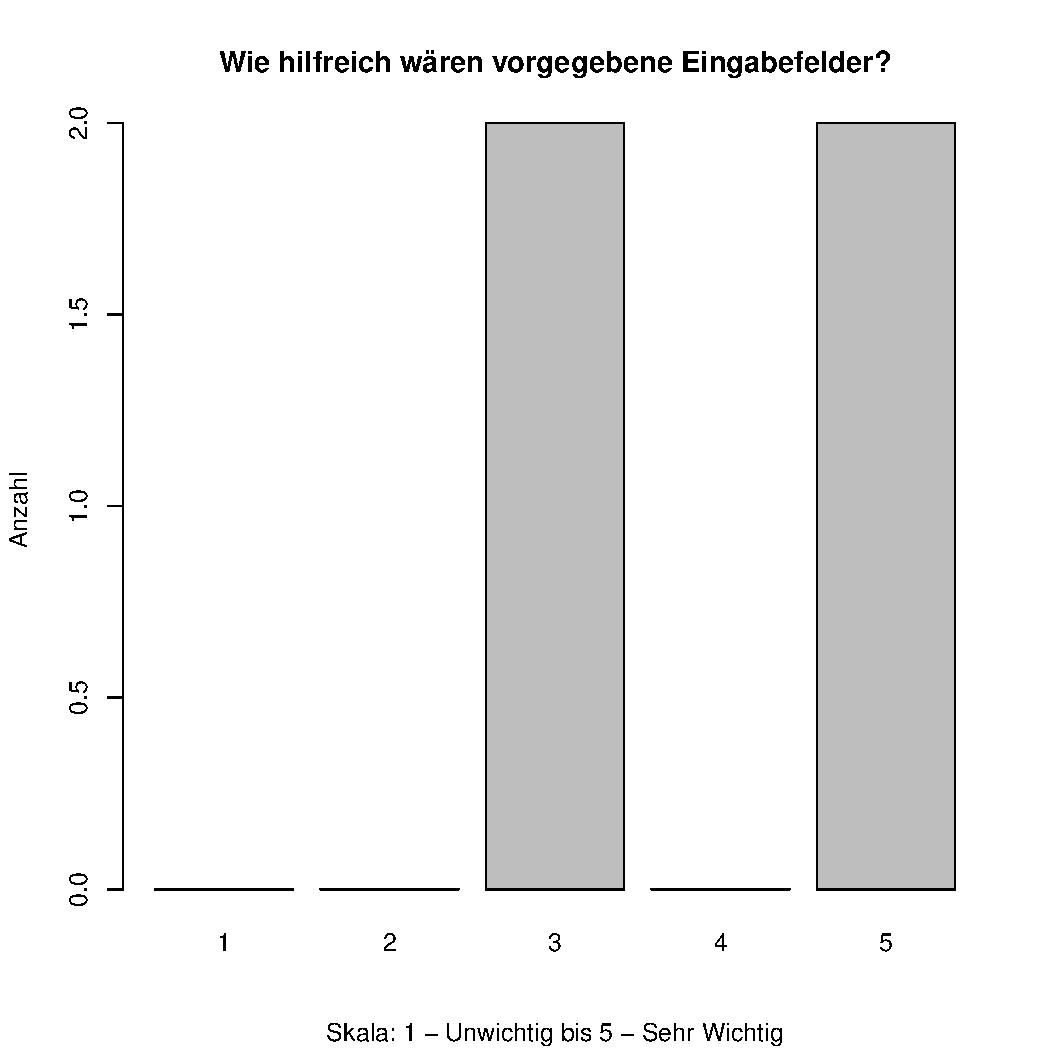
\includegraphics[width=0.60\textwidth]{q14.pdf}
    \caption{Wunsch nach Zeitbegrenzung}
	\label{fig:q14}
\end{figure} 
\section{Methodik}



